% Created by tikzDevice version 0.10.1 on 2016-08-15 16:48:02
% !TEX encoding = UTF-8 Unicode
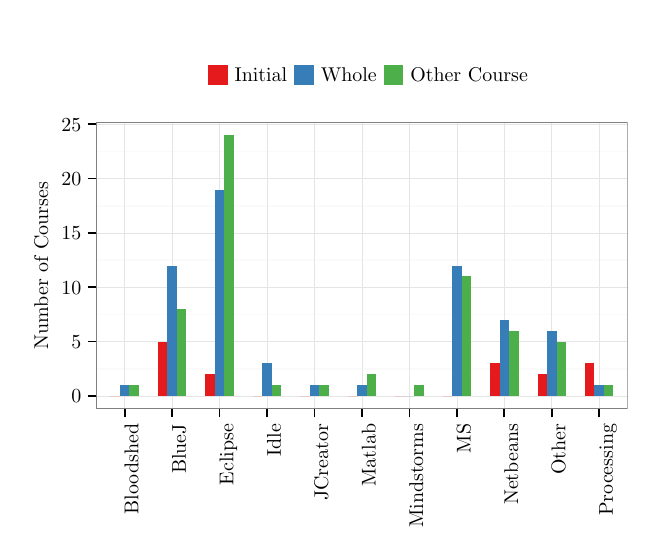
\begin{tikzpicture}[x=1pt,y=1pt]
\definecolor{fillColor}{RGB}{255,255,255}
\path[use as bounding box,fill=fillColor,fill opacity=0.00] (0,0) rectangle (216.81,180.67);
\begin{scope}
\path[clip] (  0.00,  0.00) rectangle (216.81,180.67);
\definecolor{drawColor}{RGB}{255,255,255}
\definecolor{fillColor}{RGB}{255,255,255}

\path[draw=drawColor,line width= 0.6pt,line join=round,line cap=round,fill=fillColor] (  0.00,  0.00) rectangle (216.81,180.68);
\end{scope}
\begin{scope}
\path[clip] ( 24.76, 42.89) rectangle (216.81,146.53);
\definecolor{fillColor}{RGB}{255,255,255}

\path[fill=fillColor] ( 24.76, 42.89) rectangle (216.81,146.53);
\definecolor{drawColor}{gray}{0.98}

\path[draw=drawColor,line width= 0.6pt,line join=round] ( 24.76, 57.42) --
	(216.81, 57.42);

\path[draw=drawColor,line width= 0.6pt,line join=round] ( 24.76, 77.05) --
	(216.81, 77.05);

\path[draw=drawColor,line width= 0.6pt,line join=round] ( 24.76, 96.67) --
	(216.81, 96.67);

\path[draw=drawColor,line width= 0.6pt,line join=round] ( 24.76,116.30) --
	(216.81,116.30);

\path[draw=drawColor,line width= 0.6pt,line join=round] ( 24.76,135.93) --
	(216.81,135.93);
\definecolor{drawColor}{gray}{0.90}

\path[draw=drawColor,line width= 0.2pt,line join=round] ( 24.76, 47.60) --
	(216.81, 47.60);

\path[draw=drawColor,line width= 0.2pt,line join=round] ( 24.76, 67.23) --
	(216.81, 67.23);

\path[draw=drawColor,line width= 0.2pt,line join=round] ( 24.76, 86.86) --
	(216.81, 86.86);

\path[draw=drawColor,line width= 0.2pt,line join=round] ( 24.76,106.49) --
	(216.81,106.49);

\path[draw=drawColor,line width= 0.2pt,line join=round] ( 24.76,126.12) --
	(216.81,126.12);

\path[draw=drawColor,line width= 0.2pt,line join=round] ( 24.76,145.75) --
	(216.81,145.75);

\path[draw=drawColor,line width= 0.2pt,line join=round] ( 35.05, 42.89) --
	( 35.05,146.53);

\path[draw=drawColor,line width= 0.2pt,line join=round] ( 52.19, 42.89) --
	( 52.19,146.53);

\path[draw=drawColor,line width= 0.2pt,line join=round] ( 69.34, 42.89) --
	( 69.34,146.53);

\path[draw=drawColor,line width= 0.2pt,line join=round] ( 86.49, 42.89) --
	( 86.49,146.53);

\path[draw=drawColor,line width= 0.2pt,line join=round] (103.64, 42.89) --
	(103.64,146.53);

\path[draw=drawColor,line width= 0.2pt,line join=round] (120.78, 42.89) --
	(120.78,146.53);

\path[draw=drawColor,line width= 0.2pt,line join=round] (137.93, 42.89) --
	(137.93,146.53);

\path[draw=drawColor,line width= 0.2pt,line join=round] (155.08, 42.89) --
	(155.08,146.53);

\path[draw=drawColor,line width= 0.2pt,line join=round] (172.23, 42.89) --
	(172.23,146.53);

\path[draw=drawColor,line width= 0.2pt,line join=round] (189.37, 42.89) --
	(189.37,146.53);

\path[draw=drawColor,line width= 0.2pt,line join=round] (206.52, 42.89) --
	(206.52,146.53);
\definecolor{fillColor}{RGB}{228,26,28}

\path[fill=fillColor] ( 29.90, 47.60) rectangle ( 33.33, 47.60);
\definecolor{fillColor}{RGB}{55,126,184}

\path[fill=fillColor] ( 33.33, 47.60) rectangle ( 36.76, 51.53);
\definecolor{fillColor}{RGB}{77,175,74}

\path[fill=fillColor] ( 36.76, 47.60) rectangle ( 40.19, 51.53);
\definecolor{fillColor}{RGB}{228,26,28}

\path[fill=fillColor] ( 47.05, 47.60) rectangle ( 50.48, 67.23);
\definecolor{fillColor}{RGB}{55,126,184}

\path[fill=fillColor] ( 50.48, 47.60) rectangle ( 53.91, 94.71);
\definecolor{fillColor}{RGB}{77,175,74}

\path[fill=fillColor] ( 53.91, 47.60) rectangle ( 57.34, 79.01);
\definecolor{fillColor}{RGB}{228,26,28}

\path[fill=fillColor] ( 64.20, 47.60) rectangle ( 67.63, 55.45);
\definecolor{fillColor}{RGB}{55,126,184}

\path[fill=fillColor] ( 67.63, 47.60) rectangle ( 71.06,122.19);
\definecolor{fillColor}{RGB}{77,175,74}

\path[fill=fillColor] ( 71.06, 47.60) rectangle ( 74.49,141.82);
\definecolor{fillColor}{RGB}{228,26,28}

\path[fill=fillColor] ( 81.34, 47.60) rectangle ( 84.77, 47.60);
\definecolor{fillColor}{RGB}{55,126,184}

\path[fill=fillColor] ( 84.77, 47.60) rectangle ( 88.20, 59.38);
\definecolor{fillColor}{RGB}{77,175,74}

\path[fill=fillColor] ( 88.20, 47.60) rectangle ( 91.63, 51.53);
\definecolor{fillColor}{RGB}{228,26,28}

\path[fill=fillColor] ( 98.49, 47.60) rectangle (101.92, 47.60);
\definecolor{fillColor}{RGB}{55,126,184}

\path[fill=fillColor] (101.92, 47.60) rectangle (105.35, 51.53);
\definecolor{fillColor}{RGB}{77,175,74}

\path[fill=fillColor] (105.35, 47.60) rectangle (108.78, 51.53);
\definecolor{fillColor}{RGB}{228,26,28}

\path[fill=fillColor] (115.64, 47.60) rectangle (119.07, 47.60);
\definecolor{fillColor}{RGB}{55,126,184}

\path[fill=fillColor] (119.07, 47.60) rectangle (122.50, 51.53);
\definecolor{fillColor}{RGB}{77,175,74}

\path[fill=fillColor] (122.50, 47.60) rectangle (125.93, 55.45);
\definecolor{fillColor}{RGB}{228,26,28}

\path[fill=fillColor] (132.79, 47.60) rectangle (136.22, 47.60);
\definecolor{fillColor}{RGB}{55,126,184}

\path[fill=fillColor] (136.22, 47.60) rectangle (139.65, 47.60);
\definecolor{fillColor}{RGB}{77,175,74}

\path[fill=fillColor] (139.65, 47.60) rectangle (143.08, 51.53);
\definecolor{fillColor}{RGB}{228,26,28}

\path[fill=fillColor] (149.93, 47.60) rectangle (153.36, 47.60);
\definecolor{fillColor}{RGB}{55,126,184}

\path[fill=fillColor] (153.36, 47.60) rectangle (156.79, 94.71);
\definecolor{fillColor}{RGB}{77,175,74}

\path[fill=fillColor] (156.79, 47.60) rectangle (160.22, 90.79);
\definecolor{fillColor}{RGB}{228,26,28}

\path[fill=fillColor] (167.08, 47.60) rectangle (170.51, 59.38);
\definecolor{fillColor}{RGB}{55,126,184}

\path[fill=fillColor] (170.51, 47.60) rectangle (173.94, 75.08);
\definecolor{fillColor}{RGB}{77,175,74}

\path[fill=fillColor] (173.94, 47.60) rectangle (177.37, 71.16);
\definecolor{fillColor}{RGB}{228,26,28}

\path[fill=fillColor] (184.23, 47.60) rectangle (187.66, 55.45);
\definecolor{fillColor}{RGB}{55,126,184}

\path[fill=fillColor] (187.66, 47.60) rectangle (191.09, 71.16);
\definecolor{fillColor}{RGB}{77,175,74}

\path[fill=fillColor] (191.09, 47.60) rectangle (194.52, 67.23);
\definecolor{fillColor}{RGB}{228,26,28}

\path[fill=fillColor] (201.38, 47.60) rectangle (204.81, 59.38);
\definecolor{fillColor}{RGB}{55,126,184}

\path[fill=fillColor] (204.81, 47.60) rectangle (208.24, 51.53);
\definecolor{fillColor}{RGB}{77,175,74}

\path[fill=fillColor] (208.24, 47.60) rectangle (211.67, 51.53);
\definecolor{drawColor}{gray}{0.50}

\path[draw=drawColor,line width= 0.6pt,line join=round,line cap=round] ( 24.76, 42.89) rectangle (216.81,146.53);
\end{scope}
\begin{scope}
\path[clip] (  0.00,  0.00) rectangle (216.81,180.67);
\definecolor{drawColor}{RGB}{0,0,0}

\node[text=drawColor,anchor=base east,inner sep=0pt, outer sep=0pt, scale=  0.72] at ( 19.36, 45.12) {0};

\node[text=drawColor,anchor=base east,inner sep=0pt, outer sep=0pt, scale=  0.72] at ( 19.36, 64.75) {5};

\node[text=drawColor,anchor=base east,inner sep=0pt, outer sep=0pt, scale=  0.72] at ( 19.36, 84.38) {10};

\node[text=drawColor,anchor=base east,inner sep=0pt, outer sep=0pt, scale=  0.72] at ( 19.36,104.01) {15};

\node[text=drawColor,anchor=base east,inner sep=0pt, outer sep=0pt, scale=  0.72] at ( 19.36,123.64) {20};

\node[text=drawColor,anchor=base east,inner sep=0pt, outer sep=0pt, scale=  0.72] at ( 19.36,143.27) {25};
\end{scope}
\begin{scope}
\path[clip] (  0.00,  0.00) rectangle (216.81,180.67);
\definecolor{drawColor}{RGB}{0,0,0}

\path[draw=drawColor,line width= 0.6pt,line join=round] ( 21.76, 47.60) --
	( 24.76, 47.60);

\path[draw=drawColor,line width= 0.6pt,line join=round] ( 21.76, 67.23) --
	( 24.76, 67.23);

\path[draw=drawColor,line width= 0.6pt,line join=round] ( 21.76, 86.86) --
	( 24.76, 86.86);

\path[draw=drawColor,line width= 0.6pt,line join=round] ( 21.76,106.49) --
	( 24.76,106.49);

\path[draw=drawColor,line width= 0.6pt,line join=round] ( 21.76,126.12) --
	( 24.76,126.12);

\path[draw=drawColor,line width= 0.6pt,line join=round] ( 21.76,145.75) --
	( 24.76,145.75);
\end{scope}
\begin{scope}
\path[clip] (  0.00,  0.00) rectangle (216.81,180.67);
\definecolor{drawColor}{RGB}{0,0,0}

\path[draw=drawColor,line width= 0.6pt,line join=round] ( 35.05, 39.89) --
	( 35.05, 42.89);

\path[draw=drawColor,line width= 0.6pt,line join=round] ( 52.19, 39.89) --
	( 52.19, 42.89);

\path[draw=drawColor,line width= 0.6pt,line join=round] ( 69.34, 39.89) --
	( 69.34, 42.89);

\path[draw=drawColor,line width= 0.6pt,line join=round] ( 86.49, 39.89) --
	( 86.49, 42.89);

\path[draw=drawColor,line width= 0.6pt,line join=round] (103.64, 39.89) --
	(103.64, 42.89);

\path[draw=drawColor,line width= 0.6pt,line join=round] (120.78, 39.89) --
	(120.78, 42.89);

\path[draw=drawColor,line width= 0.6pt,line join=round] (137.93, 39.89) --
	(137.93, 42.89);

\path[draw=drawColor,line width= 0.6pt,line join=round] (155.08, 39.89) --
	(155.08, 42.89);

\path[draw=drawColor,line width= 0.6pt,line join=round] (172.23, 39.89) --
	(172.23, 42.89);

\path[draw=drawColor,line width= 0.6pt,line join=round] (189.37, 39.89) --
	(189.37, 42.89);

\path[draw=drawColor,line width= 0.6pt,line join=round] (206.52, 39.89) --
	(206.52, 42.89);
\end{scope}
\begin{scope}
\path[clip] (  0.00,  0.00) rectangle (216.81,180.67);
\definecolor{drawColor}{RGB}{0,0,0}

\node[text=drawColor,rotate= 90.00,anchor=base east,inner sep=0pt, outer sep=0pt, scale=  0.72] at ( 40.00, 37.49) {Bloodshed};

\node[text=drawColor,rotate= 90.00,anchor=base east,inner sep=0pt, outer sep=0pt, scale=  0.72] at ( 57.15, 37.49) {BlueJ};

\node[text=drawColor,rotate= 90.00,anchor=base east,inner sep=0pt, outer sep=0pt, scale=  0.72] at ( 74.30, 37.49) {Eclipse};

\node[text=drawColor,rotate= 90.00,anchor=base east,inner sep=0pt, outer sep=0pt, scale=  0.72] at ( 91.45, 37.49) {Idle};

\node[text=drawColor,rotate= 90.00,anchor=base east,inner sep=0pt, outer sep=0pt, scale=  0.72] at (108.59, 37.49) {JCreator};

\node[text=drawColor,rotate= 90.00,anchor=base east,inner sep=0pt, outer sep=0pt, scale=  0.72] at (125.74, 37.49) {Matlab};

\node[text=drawColor,rotate= 90.00,anchor=base east,inner sep=0pt, outer sep=0pt, scale=  0.72] at (142.89, 37.49) {Mindstorms};

\node[text=drawColor,rotate= 90.00,anchor=base east,inner sep=0pt, outer sep=0pt, scale=  0.72] at (160.04, 37.49) {MS};

\node[text=drawColor,rotate= 90.00,anchor=base east,inner sep=0pt, outer sep=0pt, scale=  0.72] at (177.19, 37.49) {Netbeans};

\node[text=drawColor,rotate= 90.00,anchor=base east,inner sep=0pt, outer sep=0pt, scale=  0.72] at (194.33, 37.49) {Other};

\node[text=drawColor,rotate= 90.00,anchor=base east,inner sep=0pt, outer sep=0pt, scale=  0.72] at (211.48, 37.49) {Processing};
\end{scope}
\begin{scope}
\path[clip] (  0.00,  0.00) rectangle (216.81,180.67);
\definecolor{drawColor}{RGB}{0,0,0}

\node[text=drawColor,rotate= 90.00,anchor=base,inner sep=0pt, outer sep=0pt, scale=  0.72] at (  7.36, 94.71) {Number of Courses};
\end{scope}
\begin{scope}
\path[clip] (  0.00,  0.00) rectangle (216.81,180.67);
\definecolor{fillColor}{RGB}{255,255,255}

\path[fill=fillColor] ( 56.56,155.07) rectangle (185.01,172.14);
\end{scope}
\begin{scope}
\path[clip] (  0.00,  0.00) rectangle (216.81,180.67);
\definecolor{fillColor}{RGB}{228,26,28}

\path[fill=fillColor] ( 65.15,160.05) rectangle ( 72.26,167.16);
\end{scope}
\begin{scope}
\path[clip] (  0.00,  0.00) rectangle (216.81,180.67);
\definecolor{fillColor}{RGB}{55,126,184}

\path[fill=fillColor] ( 96.30,160.05) rectangle (103.41,167.16);
\end{scope}
\begin{scope}
\path[clip] (  0.00,  0.00) rectangle (216.81,180.67);
\definecolor{fillColor}{RGB}{77,175,74}

\path[fill=fillColor] (128.64,160.05) rectangle (135.75,167.16);
\end{scope}
\begin{scope}
\path[clip] (  0.00,  0.00) rectangle (216.81,180.67);
\definecolor{drawColor}{RGB}{0,0,0}

\node[text=drawColor,anchor=base west,inner sep=0pt, outer sep=0pt, scale=  0.72] at ( 74.78,161.12) {Initial};
\end{scope}
\begin{scope}
\path[clip] (  0.00,  0.00) rectangle (216.81,180.67);
\definecolor{drawColor}{RGB}{0,0,0}

\node[text=drawColor,anchor=base west,inner sep=0pt, outer sep=0pt, scale=  0.72] at (105.93,161.12) {Whole};
\end{scope}
\begin{scope}
\path[clip] (  0.00,  0.00) rectangle (216.81,180.67);
\definecolor{drawColor}{RGB}{0,0,0}

\node[text=drawColor,anchor=base west,inner sep=0pt, outer sep=0pt, scale=  0.72] at (138.27,161.12) {Other Course};
\end{scope}
\end{tikzpicture}
